\documentclass{book}

\usepackage{fullpage}

%\usepackage{wrapfig}
%\usepackage{float}
%  \floatstyle{ruled}
%  \newfloat{callout}{thp}{lop}
%  \floatname{callout}{Things To Remember}

\usepackage{color}
\definecolor{Light}{gray}{.95}

\usepackage{amsthm}
{
  \theoremstyle{definition}
  \newtheorem{example}{Example}
}

\usepackage{graphicx}

\newlength{\calloutparindent}
\setlength{\calloutparindent}{\parindent}
%%
%% begin: the callout command
\newcommand{\callout}[3]{\label{#1}\vspace{3mm}
\begin{center}
\fcolorbox{black}{Light}{\begin{minipage}{0.85\textwidth}
    \textbf{\large Things To Remember~\ref{#1} --- #2}
    \hrule
    \vspace{2mm}
\setlength{\parindent}{\calloutparindent}
#3
  \end{minipage}}
\end{center}
\vspace{3mm}
}
\newcommand{\thingstoremember}[1]{Things To Remember~\ref{#1}}
%% end: the callout command
%%

% two chapters will precede the one here now
\setcounter{chapter}{2}

\begin{document}

\chapter{Memory Health}

A data structure may be big, but how do you know if it is too big? This chapter introduces the concept of memory health, a way to gauge how efficiently a data structure uses memory. Java developers often have to piece together many smaller objects to build a single data structure. Memory health is a way to understand the overhead introduced in each object, the impact of connecting these objects into larger data structures, and, finally, how a data structure scales as the amount of data it holds grows. Understanding memory health can provide valuable insight into each step of the data modeling process.

Later chapters show how to estimate both the size and health of data structure designs. Both of these are important. Memory health is independent of size: a small structure can be unhealthy, and a large structure can be healthy. A healthy data structure will generally scale well, while unhealthy data structures are often the root causes of memory footprint problems. 

%The examples .

\section{Distinguishing Data from Overhead}

The size of a data structure is the number of bytes it occupies. The \emph{health} of a data structure tells you what these bytes are accomplishing. Is the memory being spent on something important?  A very useful way to classify bytes is as either data or overhead. Bytes classified as data represent the real data intrinsic to your program. All other bytes are overhead of the particular representation you have chosen for that data. A healthy data structure, from a space standpoint, is one with a low overhead.  Sometimes there are tradeoffs; a larger design may be necessary for performance. Sometimes, though, choosing a design with lower memory overhead actually improves performance.

In Java, it is all too easy to design a data structure that is bloated by a factor of more than 50\%; this means that over half of the data structure is devoted to things unrelated to the data that the application cares about. To understand why there is so much overhead, it is useful to dig deeper into its different sources:  
\begin{itemize}
\item \emph{JVM overhead.} Each object has a header imposed by the JVM to facilitate various administrative tasks, such as garbage collection. In addition, the JVM may impose additional object alignment overhead.
\item \emph{Pointers}. Pointers glue objects together into data structures. Pointers can be null or non-null.   
\item \emph{Bookkeeping fields}. Not all primitive fields store real application data. Some are bookkeeping fields needed by the representation. 
\end{itemize}


\callout{callout:memory-bloat-factor}{The Memory Bloat Factor}{
    An important metric for evaluating the health of a data model
    design is the fraction of overhead in the objects of that data
    model. The \emph{memory bloat factor}, or simply \emph{bloat
      factor}, is the ratio of overhead to total size. 
}
% TODO: add alignment
\begin{figure}
  \centering
  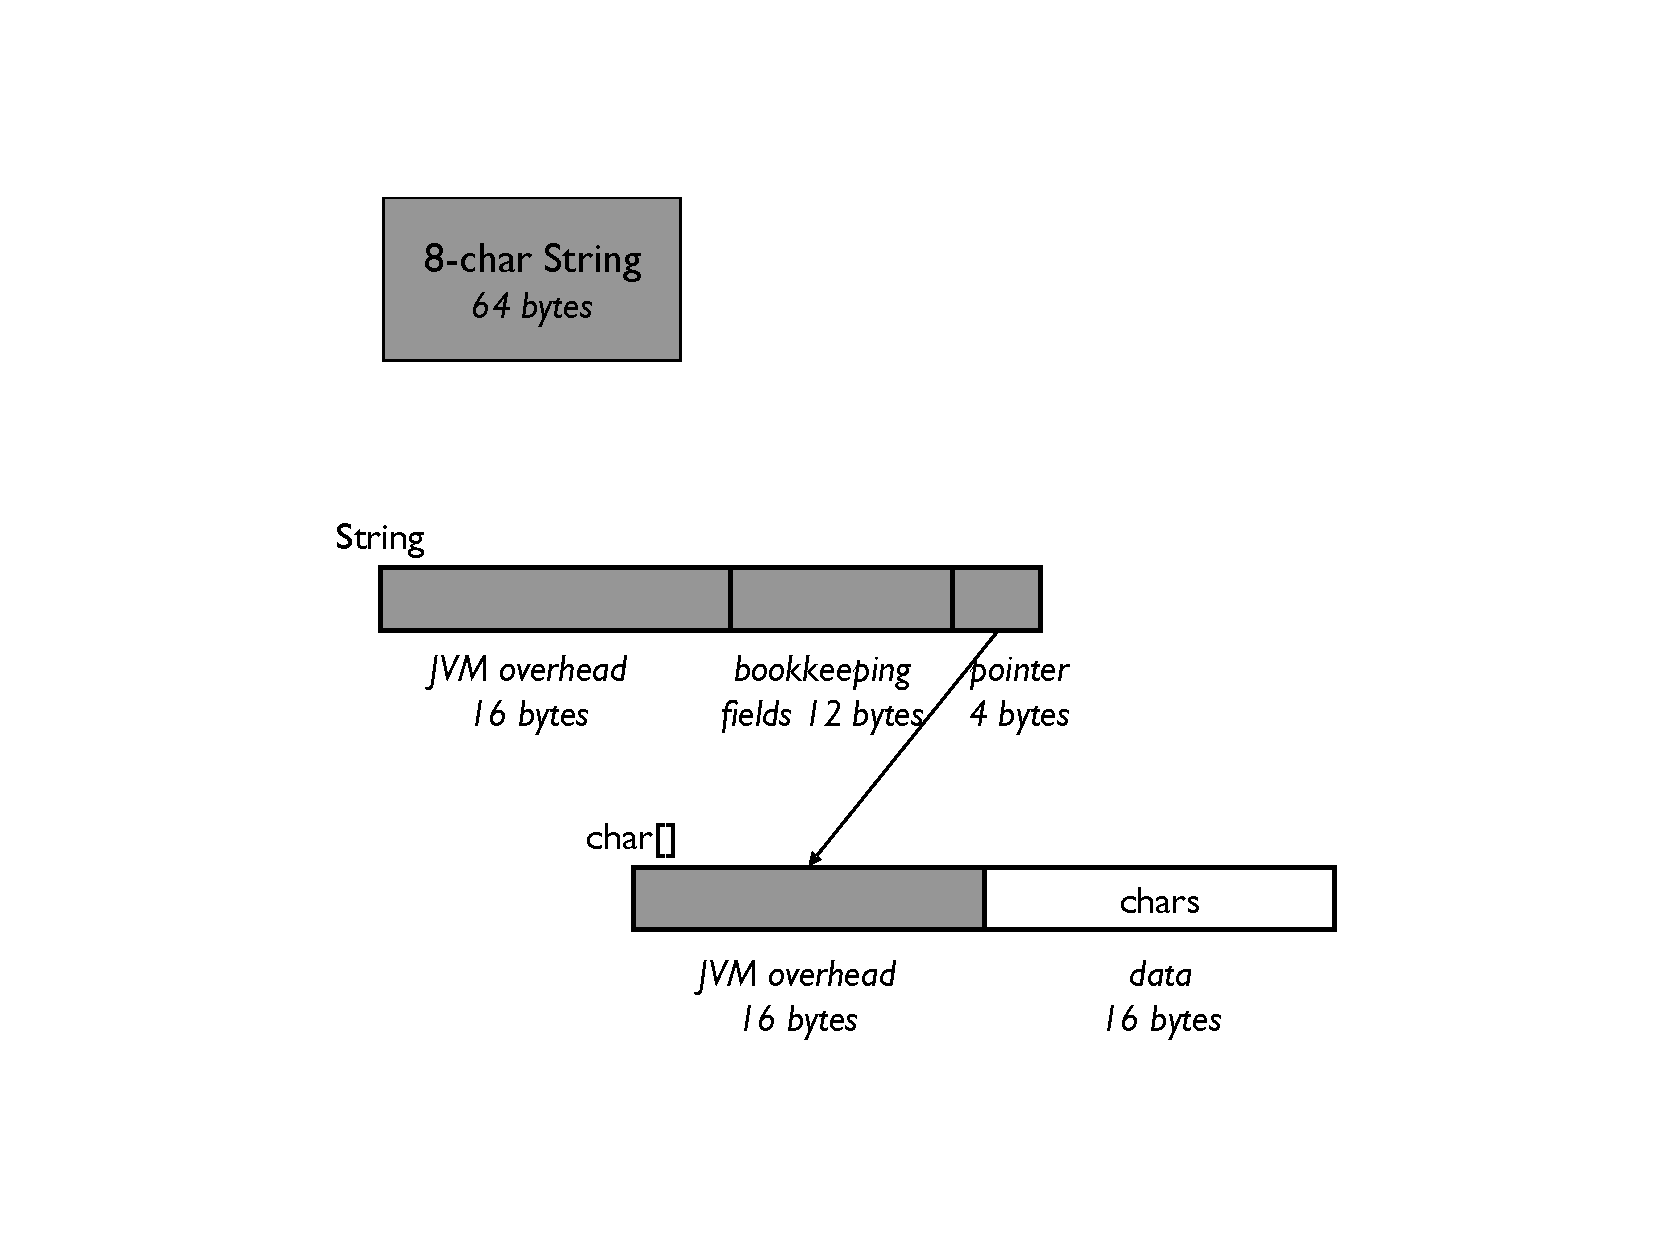
\includegraphics[width=.70\textwidth]{Figures/chapter3/eight-char-string.pdf}
  %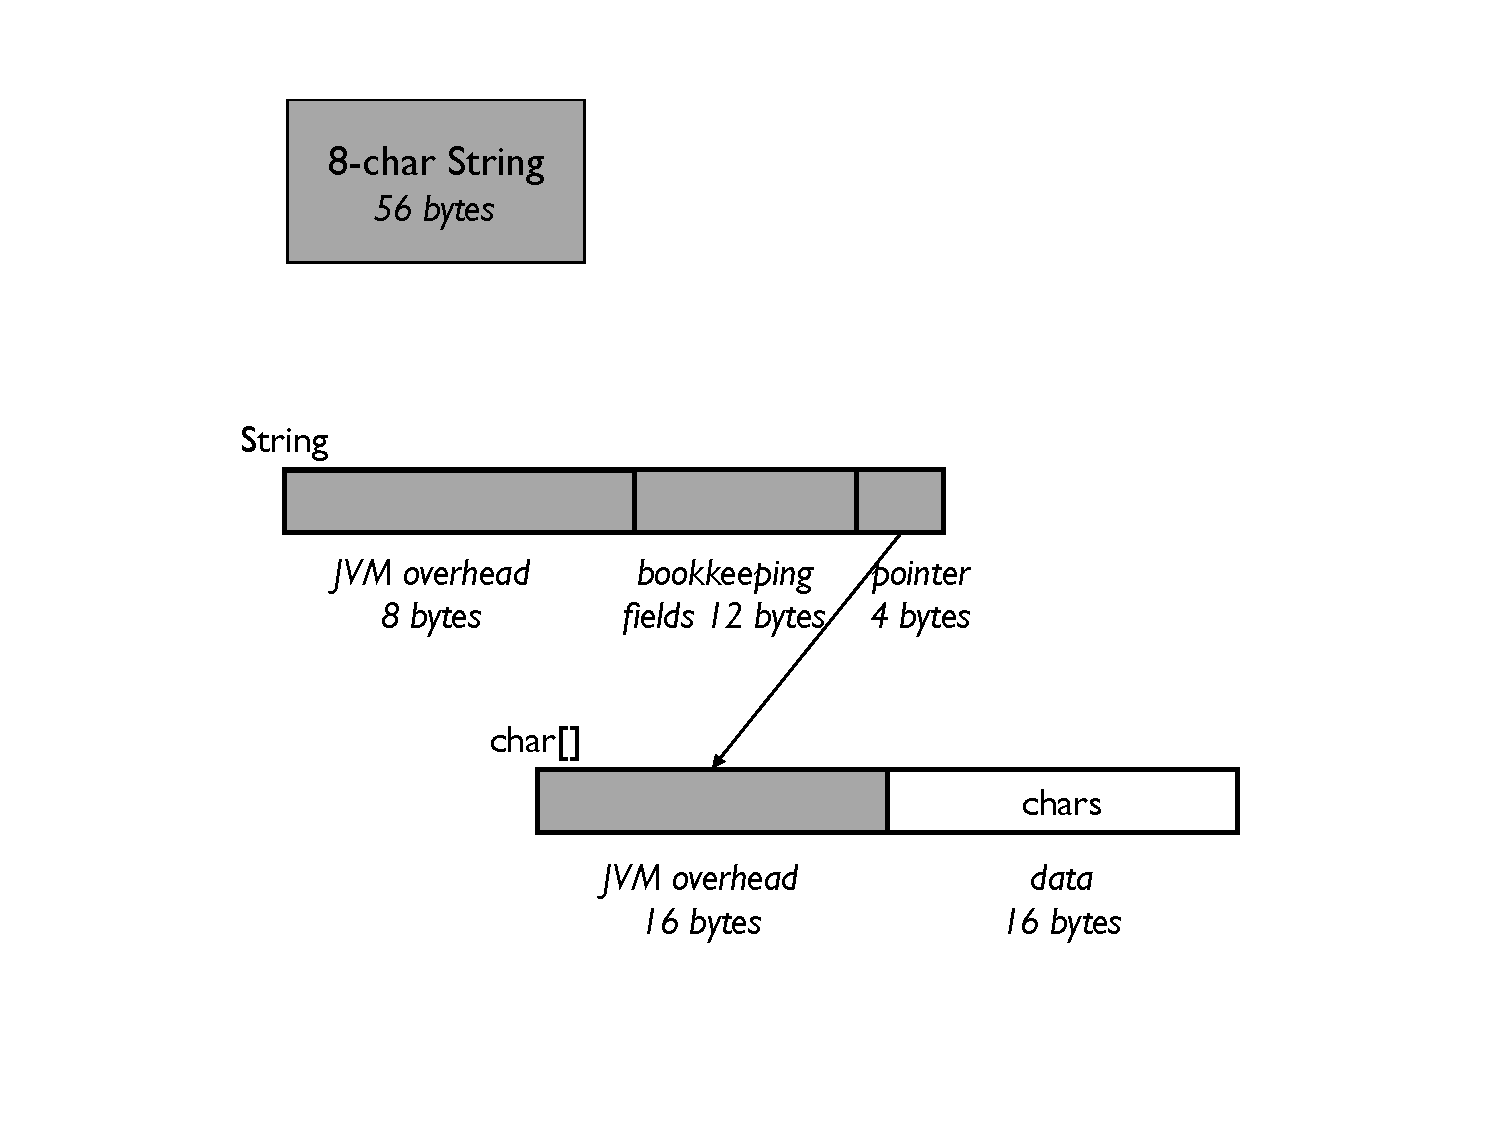
\includegraphics{eight-char-string}
  \caption{An eight character string in Java 6.}
  \label{fig:eight-char-string}
\end{figure}

\begin{example}[An 8-Character String]
 You learned in the quiz in Chapter 2 that an 8-character string occupies 64 bytes, which seems surprisingly high. The actual character data takes up 16 bytes, since Java supports the international character set, which uses 2-bytes per character. So it costs 16 bytes to represent the eight characters themselves. The other 48 bytes are pure overhead. This structure has a \emph{bloat factor} of 75\%. The actual data occupies only 25\%. These numbers vary from one JVM to another, but the overhead is always very high. (Unless otherwise noted, all measurements in this book are from the 32-bit IBM Java 6 JVM.)

Figure~\ref{fig:eight-char-string} shows why the bloat factor is so high. Strings have all three kinds of overhead -- JVM overhead, pointers, and bookkeeping fields. Every Java string is really two objects: a {\tt String} that serves as a wrapper, and a {\tt char} array with the actual characters. Two objects means two object headers, plus the pointer glueing the two objects together. The {\tt String} object is entirely overhead, containing no real data. Part of its cost is three bookkeeping fields: a length and an offset, which have meaning only when this string is the result of a substring operation, and a saved hashcode. Adding all of this together, the overhead is 48 bytes.  
\end{example}
If you were to design a string from scratch, 20\%
overhead might seem a reasonable target. For such a common data type, it is important to obtain a low overhead.
Unfortunately, for a string to have only 20\% overhead with its current implementation, it would need
to be 96 characters long. As bad as this seems, this string
representation does at least have the benefit that it amortizes away
its overhead. The overhead cost is always 48 bytes, so overhead of a string approaches 0\% for larger and larger strings.  For some data structures it is not possible to
amortize away overhead costs, as discussed in
Section~\ref{scalability}.

Strings, in particular short strings, are pervasive. It is important to be aware of the overhead of strings when incorporating them into your data design. Given the overhead of Java strings, the choices you make in Java need to be different than in a language like C, where the string overhead is minimal. Making informed choices is critical for the overall memory health of an application. There will be more on strings in later chapters.

\section{Entities and Collections}

A string is an example of a very simple data structure.  When
modeling a more complex data structure, you design classes to
represent application entities, and choose collections in which to
store them. Seemingly small choices you make in both cases can have a
big impact in memory bloat. For example, the choice of the initial
capacity of a collection can make or break the scalability of your
design. 
%The memory health approach looks at entities and collections
%separately, since there are different kinds of choices and pitfalls in
%each.

To help understand the health of more complex data structures, it is
useful to have a diagram notation that spells out the impacts of various choices.  An Entity-Collection (EC) diagram is a cousin of an Entity-Relation (ER) diagram, that exposes just the right level of implementation detail to help calculate the memory bloat
factor of a complex data structure. As its name implies, an EC diagram shows the entities and collections of a design. It is important to remember that the entities and collections in the diagram are abstracted from the actual data structure objects. A diagram box may be hiding other objects that help implement the entity or collection. For example, a diagram box for a \texttt{String} entity represents both the \texttt{String} object and its underlying character
array. 

\callout{callout:ec-diagram}{The Entity-Collection (EC) Diagram}{

\begin{center}
  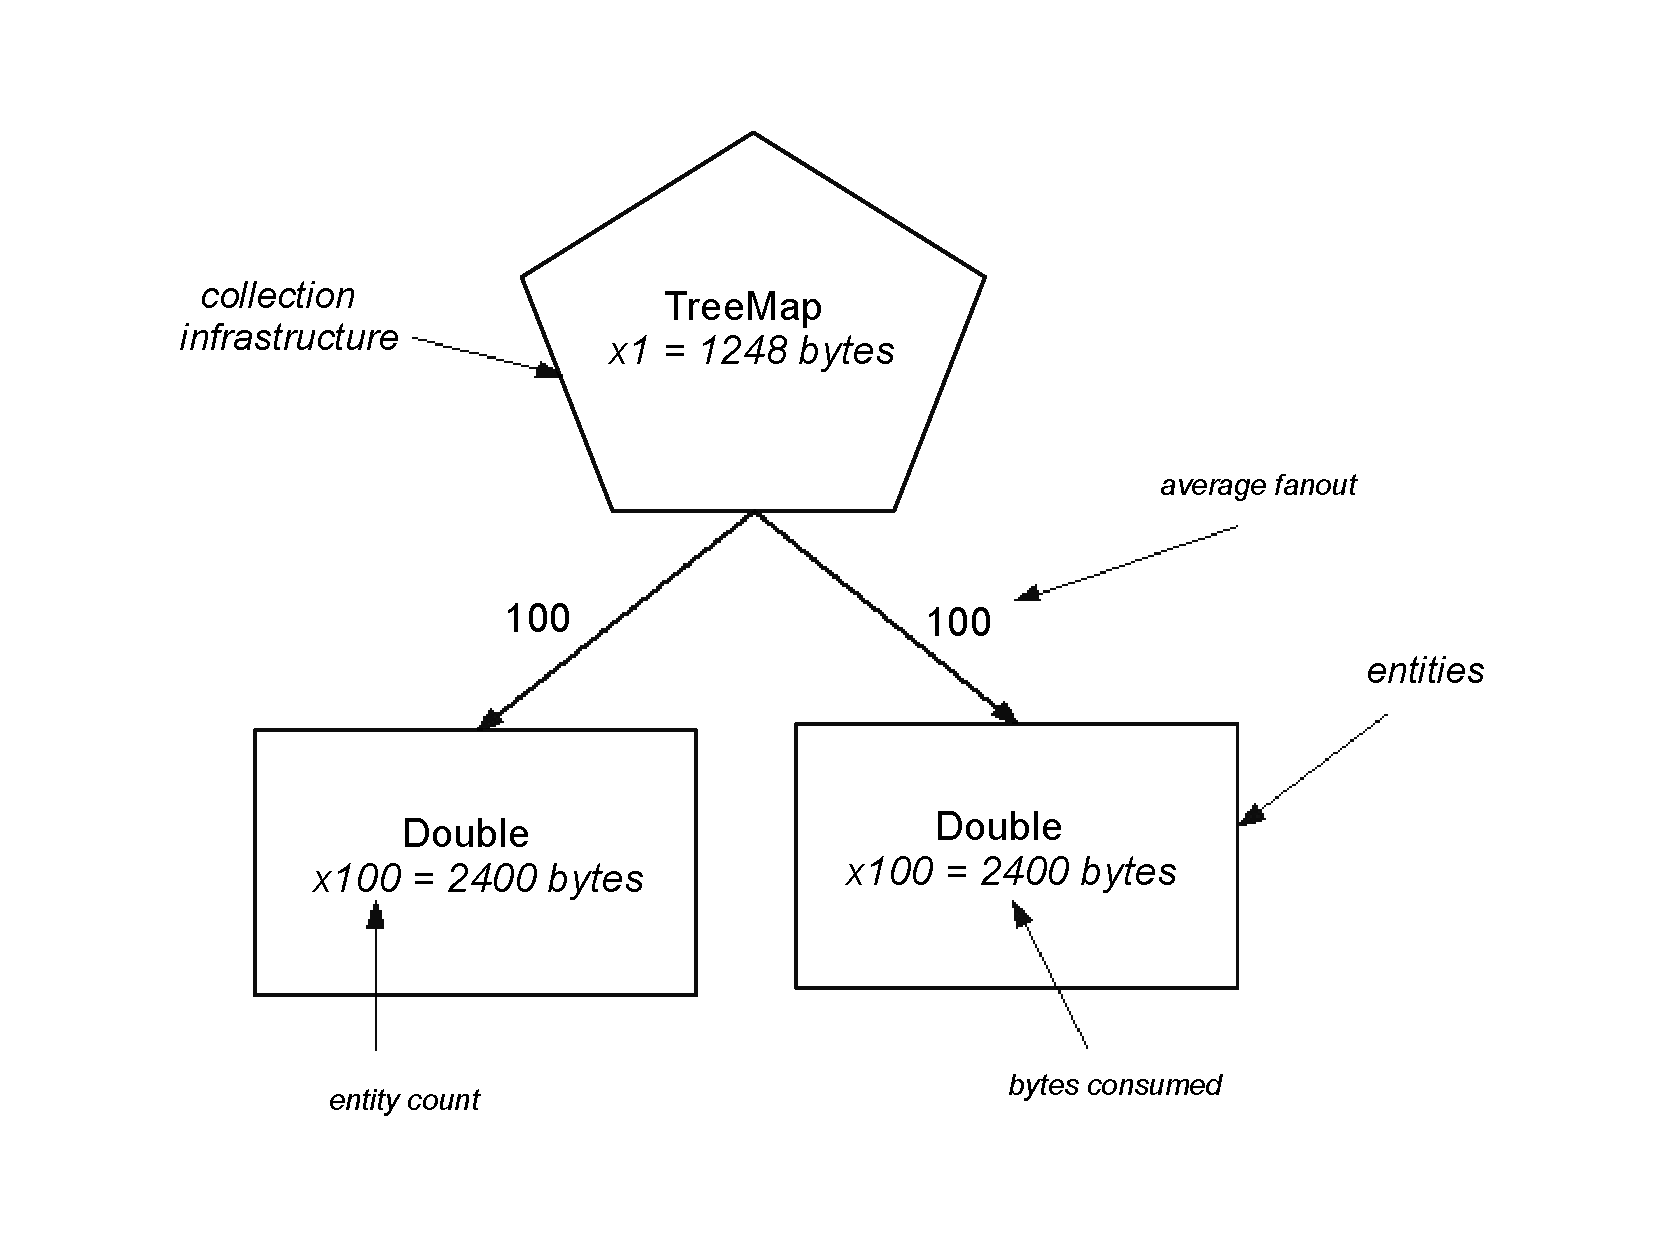
\includegraphics[width=0.7\textwidth]{Figures/chapter3/content-schematic}
\end{center}

In an EC diagram, there are two types of boxes, pentagons and
rectangles. Each box summarizes the implementation details of a portion
of a data structure.  Pentagons represent collection infrastructure,
and rectangles represent the entities of your application.

An EC diagram represents the {\em containment} structure of your data
model. So, an edge from a collection to a rectangular entity indicates
membership of the entity in the collection. This also means that, if a
certain type of collection or entity is used in multiple ways in the
same data structure, then this type will appear in multiple locations
--- one in each location in the data structure in which that type is
used.

The notation $x N = M$ inside each node means there are $N$
objects of that type in that location in the data structure, and in
total these objects occupy $M$ bytes of memory. Each edge in a
content schematic is labeled with the average fanout from the source
entity to the target entity.
%\caption{--- The Entity-Collection (EC) Diagram}

%Notice how an EC diagram summarizes away some of the details that an
%ER diagram shows, and shows some implementation details than an ER
%diagram does not include.
%The EC diagram represents collection choices, rather than the
%relations they implement.
%where an ER diagram would show a single relation node for an M-to-N
%relation, 
Where an ER or UML diagram would show the attributes of each entity,
but ignore the implementation costs, an EC diagram summarizes the
total cost in the single sizing number shown in each node. Where these other diagrams
would show relations or roles as edges, an EC diagram shows a node summarizing the
collections implementing this relation.
%Unlike UML diagrams, relationships are elevated to be entities, rather
%than edges. The reason is that in a language like Java, implementation
%of the relationship itself is often a big cause of expense, so it is
%important to make that visible. A very common pattern is to implement
%relationships as collections. 
 }

%%%% this is the old Collection of Strings example
%In Figure~\ref{fig:content-schematic}, there are two
%\texttt{Collection}s which together occupy 200 bytes, and ten
%\texttt{String}s occupy 880 bytes. There are on average five elements
%contained in each of the two \texttt{Collection}. Since the overhead
%of a \texttt{String} is 48 bytes and there are 10 \texttt{String}s,
%the total overhead is 480 bytes or 55\%. Data occupies 400 bytes, so
%the average \texttt{String} length is 10. The two \texttt{Collection}s
%are pure overhead, so the total overhead of this data structure is 680
%bytes, or 63\%.



% The name of an entity is the name of the top object. Entities also
% summarize objects of the same type that are repeated in a data
% structure. The \texttt{String} entity in
% Figure~\ref{fig:content-schematic} represents the 10 \texttt{String}s
% in the two \texttt{Collection}s. The memory cost of an entity is the
% sum over all of its objects. This summarization removes clutter and
% helps understanding.

%\begin{figure}
%  \centering
%  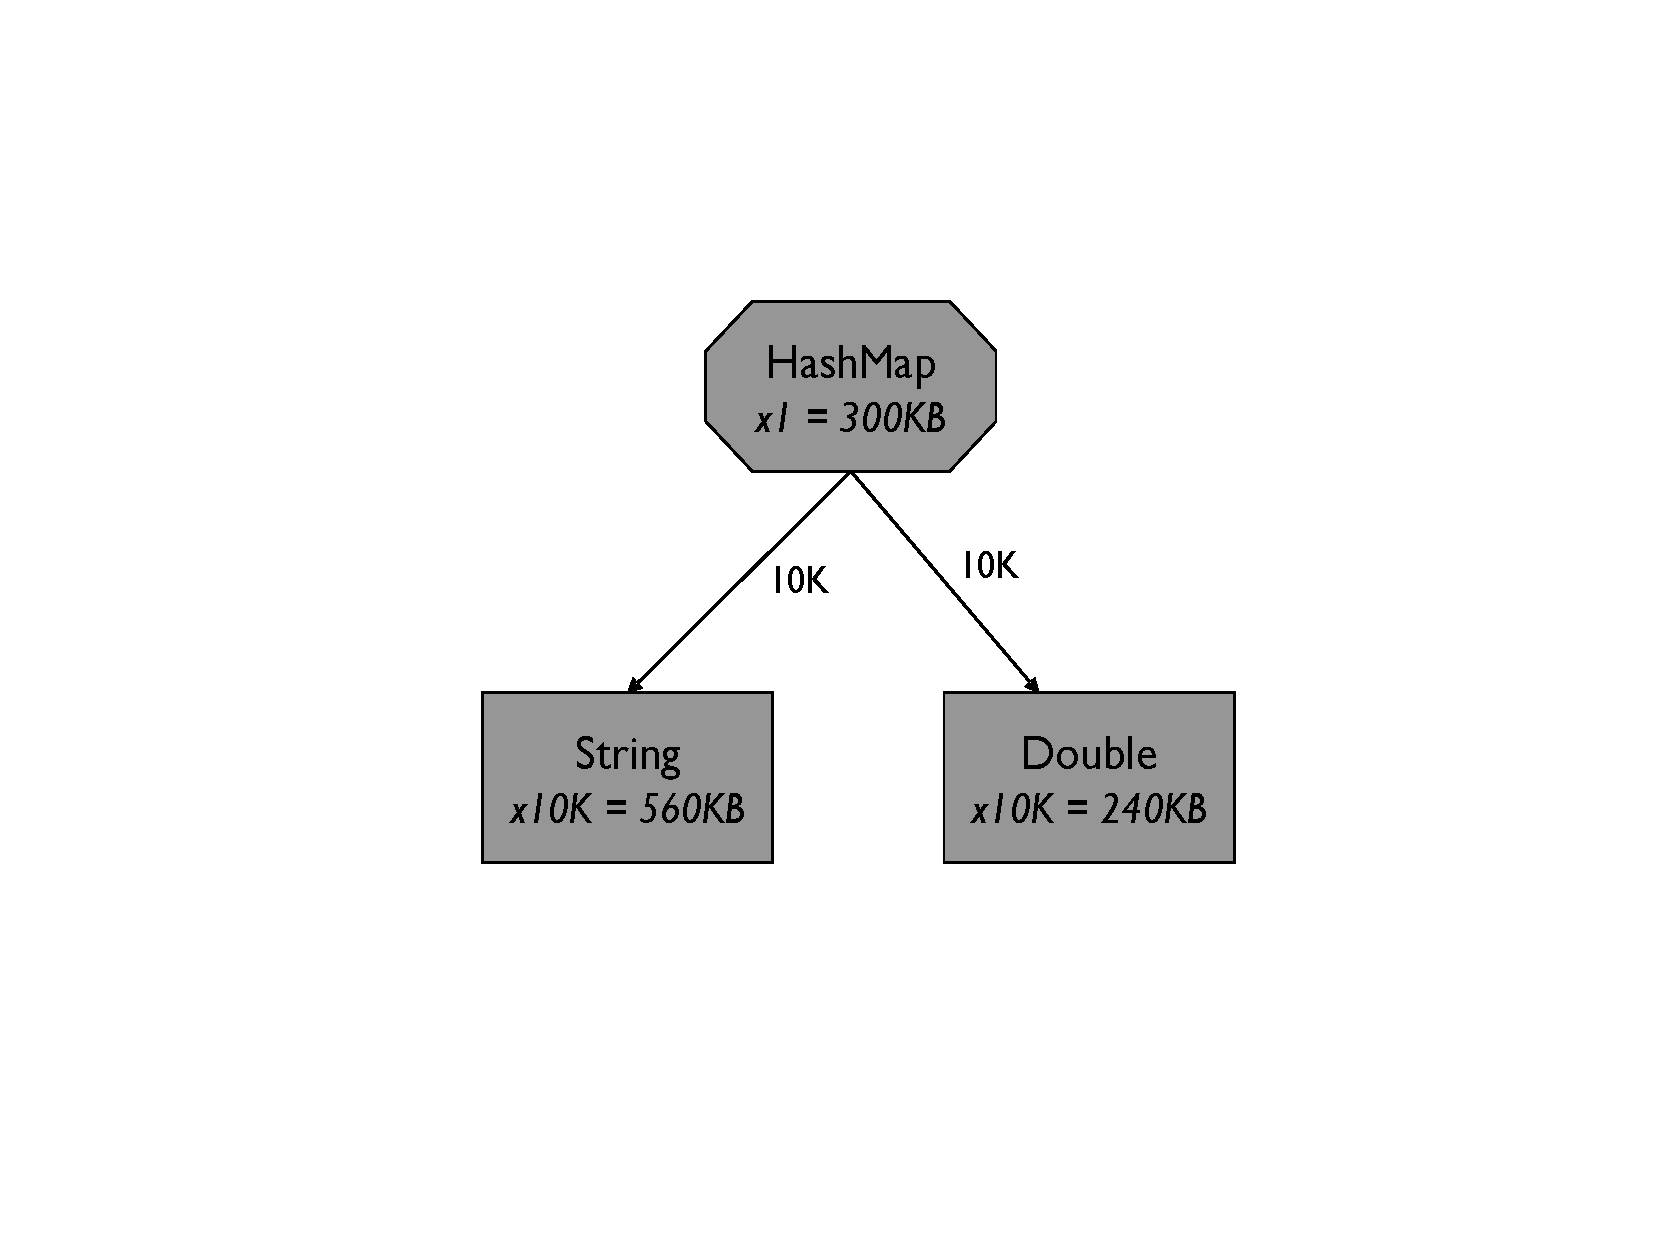
\includegraphics[width=0.9\textwidth]{Figures/content-schematic-relationship}
%  \caption{A content schematic of a map from 10K \texttt{Strings} to 10K \texttt{Doubles}.}
 % \label{fig:content-schematic-relationship}
%\end{figure}



%\section{Example: Sorted Map of Doubles}
%\label{section:mapofdoubles}

 \begin{example}[A Monitoring System]
   A monitoring program collects samples from a distributed
   system. Each sample it collects consists of a unique timestamp and a
   value, each represented as a double. The samples arrive out of
   order. The task is to display samples in chronological order, after
   all of the data has been collected. The solution requires a data
   structure to store the samples. 
\end{example}
%\emph{Load-and-Use Behavior Pattern:} load data in one phase, use the data in the next phase.


A map is a convenient way to store these timestamp-value pairs. A regular \texttt{HashMap} only solves part of the monitoring system problem. To be able to display the samples in chronological order, the entries have to be sorted by timestamp. 
The first idea that leaps forward is to use a \texttt{TreeMap}. A \texttt{TreeMap} is a map that maintains its entries in sorted order, so this appears to be a perfect choice. The only problem is the memory cost.

An EC diagram of a \texttt{TreeMap} storing 100 samples is shown in Figure~\ref{fig:content-schematic-treemap-doubles}.  This diagram gives a schematic view of the \texttt{TreeMap} and the entities it contains, along with their costs. The total cost, obtained by adding up the entity and collection costs, is 6,048 bytes. The real data consumes only 1,600 bytes of this, since a double occupies 8 bytes and there are 200 of them. Therefore, the bloat factor is 74\%.  

\begin{figure}
  \centering
  %\includegraphics[width=0.4\textwidth]{Figures/treemap-doubles}
  \includegraphics[width=0.7\textwidth]{Figures/chapter3/treemap-doubles}
  \caption{EC Diagram for 100 samples stored in a \texttt{TreeMap}}
  \label{fig:content-schematic-treemap-doubles}
\end{figure} 
 
Looking at the individual parts of the EC diagram can provide some insight into the source of this overhead. First, the sample timestamps and values are stored as \texttt{Double} objects. This is because the standard Java collection APIs take only \texttt{Object}s as parameters, not scalars, forcing you to box your scalars before putting them in a collection. Even with Java's autoboxing, the compiler still generates a boxed scalar in order to store a value in a standard collection.  A single instance of a \texttt{Double} is 24 bytes, so 200 \texttt{Doubles} occupy 4,800 bytes. Since the data is only 1,600 bytes,  33\% of the \texttt{Double} objects is actual data, and 67\% is overhead. This is a high price for a basic data type. 

%A double occupies eight bytes, each sample has two doubles, so 100 samples occupy 1.6KB of actual data  -- put this into the diagramf

%Move this later? At best, the overhead will be 67\% if the doubles are boxed.

The \texttt{TreeMap} infrastructure occupies an additional 1,248 bytes of memory. All of this is overhead. What is taking up so much space?  \texttt{TreeMap}, like every other collection in Java, has a wrapper object, the \texttt{TreeMap} object itself, along with other internal objects that implement the collection functionality. Each type of collection in the standard library has a different kind of infrastructure, some are built from arrays, some from separate entry objects linked together, and some use a combination of both. Internally, \texttt{TreeMap} is a self-balancing search tree. The tree nodes maintain pointers to parents and siblings.  In newer releases of Java 6, each node in the tree can store up to 64 key-value pairs in two arrays. This example uses this newer implementation, which is more memory-efficient for this case, but still expensive. 
%    there is a separate \texttt{Treemap\$Entry} object. This is typical of collections. A typical collection has a fixed overhead, in this case it is 48 bytes, and a per-entry overhead cost, in this case it is 40 bytes per entry. These 40 bytes include five pointer fields, in addition to other sources of overhead. 

Using a \texttt{TreeMap} is not \textit{a priori} a bad design. It depends on whether the overhead is buying something useful. \texttt{TreeMap} has a high memory cost because it maintains its entries in sorted order while they are being randomly inserted and deleted. It constantly maintains a sorted order. If you need this capability, for instance, if you have a real time monitor that is constantly being updated, and you need to look at the data in order, then \texttt{TreeMap} is a great data structure.  But if you do not need this capability, there are other data structures that could provide sorted-map functionality with less memory consumption. In this example, the data needs to be sorted only after data collection is complete. There is an initial load phase followed by a use phase. The sorted order is only needed during the second phase, after all the data is loaded. This load-and-use behavior is a common pattern, and it can be exploited to choose a more memory-efficient representation.

Of course, another nice aspect of \texttt{TreeMap} is that it can be pulled off the shelf. It would be ideal if there were another collection that provides just the needed functionality. If not, maybe there is a way to easily extend another collection class by adding a thin wrapper around it. Writing your own collection class from scratch should rarely be necessary, and is not recommended.

\section{Two Memory-Efficient Designs}
\label{better-designs} 

This section describes two other data structure designs to store the monitoring system samples. These designs use less memory and do not maintain sorted order while the data is being loaded. This is not a problem, since the data can be sorted after loading. 

The first design stores the samples in an \texttt{ArrayList}, where each entry is a \texttt{Sample} object containing a timestamp and value. Both values are stored in primitive \texttt{double} fields of \texttt{Sample}.  There is a bit more code that has to be written, but it is not excessive. Fortunately, the standard Java \texttt{Collections} class has some useful static methods so that new sort and search algorithms do not have to be implemented. The \texttt{sort} and \texttt{binarySearch} methods from \texttt{Collections} each can take an \texttt{ArrayList} and a \texttt{Comparable} object as parameters. To take advantage of these methods, the new \texttt{Sample} class has to implement the \texttt{Comparable} interface, so that two sample timestamps can be compared:  

\ttfamily
\begin{verbatim}
   
    public class Sample implements Comparable<Sample> {

        private final double timestamp;
        private final double value;
	
        public Sample(double timestamp, double value) {
            this.timestamp = timestamp;
            this.value = value;
        }
	
        public double getTimestamp() {
            return timestamp;
        }
	
        public double getValue() {
            return value;
        }
	      
        public int compareTo(Sample that) {
            return Double.compare(this.getTimestamp(), that.getTimestamp());	
        }
    }

\end{verbatim}
\normalfont
Additionally, the \texttt{ArrayList} needs to be stored in a wrapper class that implements map operations. Here are two methods, \texttt{getValue} and \texttt{sort}, of a wrapper class \texttt{Samples}. 
\ttfamily
\begin{verbatim}
    public class Samples {
    
    	  public final static double NOT_FOUND = -1d;
        private ArrayList<Sample> samples = new ArrayList<Sample>();
        ....
		
        public double getValue(double timestamp) {
            Sample sample = new Sample(timestamp, 0.0);
            int result = Collections.binarySearch(samples, sample);
            if (result < 0) {
            	return NOT_FOUND;
            }
            return samples.get(result).getValue();
        }
		
        public void sort() {
            Collections.sort(samples);
            samples.trimToSize();	
        }
    }
    
\end{verbatim}
\normalfont 
  
The EC diagram for 100 entries is shown in Figure~\ref{fig:content-schematic-arraylist-pairs}.
\begin{figure}
  \centering
 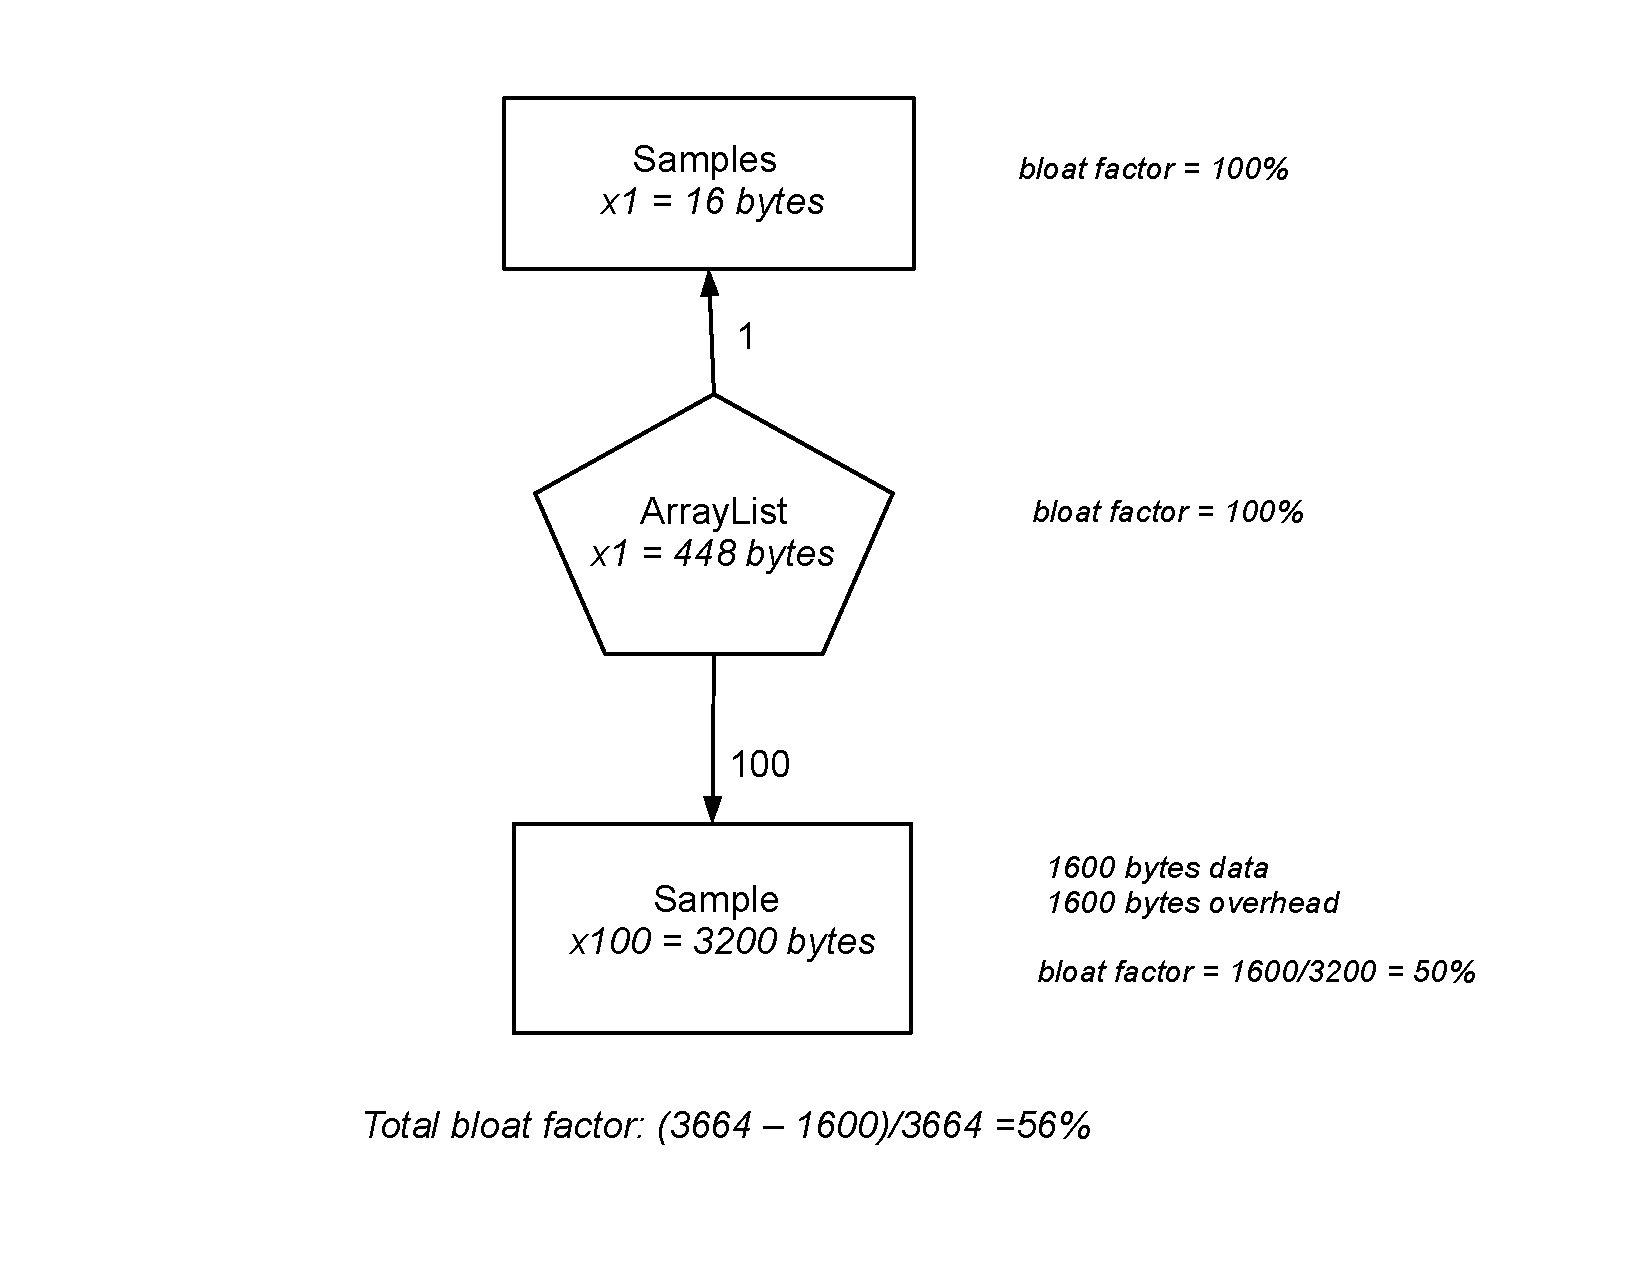
\includegraphics[width=0.7\textwidth]{Figures/chapter3/arraylist-doubles}
  \caption{EC Diagram for 100 samples stored in an \texttt{ArrayList} of \texttt{Samples}}
  \label{fig:content-schematic-arraylist-pairs}
\end{figure} 
This design uses less memory and has better health than the \texttt{TreeMap} design. The memory cost is reduced from 6,048 to 3,664 bytes, and the overhead is reduced from 74\% to 56\%.  There are two reasons for this improvement. First, the timestamps and values are not boxed. They are stored as primitive double fields in each \texttt{Sample}. This reduces the number of objects needed to store the actual data from 200 to 100. Fewer objects means fewer object headers and pointers, which is significant in this case. Secondly, an \texttt{ArrayList} has lower infrastructure cost than a \texttt{TreeMap}. \texttt{ArrayList} is one of the most memory-efficient Java collections. It is implemented using a wrapper object and an array of pointers. This is much more compact than the heavy-weight \texttt{TreeMap}. 

While this is a big improvement, 56\% overhead still seems high. Over half the memory is being wasted. How hard is it to get rid of this overhead completely? Eliminating overhead means eliminating objects altogether. This is not a recommended practice, unless memory is extremely tight, and there is no other choice. It is none the less an interesting exercise to compare a best case design with the other designs. The most space-efficient design uses two parallel arrays of doubles. One array stores all of the sample timestamps, and the second stores all of the values. These arrays can be stored in a wrapper class that implements a map interface.

This design requires a bit more code, but, again, it is not excessive. Like the \texttt{Collections} class, the \texttt{Arrays} class provides static \texttt{sort} and  \texttt{binarySearch} methods. However, these methods apply only to a single array. If you sort the timestamp array, you will lose the association between the timestamps and their corresponding values. You can use an extra temporary array to get around this problem. The implementation is left as an exercise. The EC diagram for this design using two double arrays is shown in 
Figure~\ref{fig:content-schematic-arrays-doubles}. The overhead is only 4\%. 

\begin{figure}
  \centering
  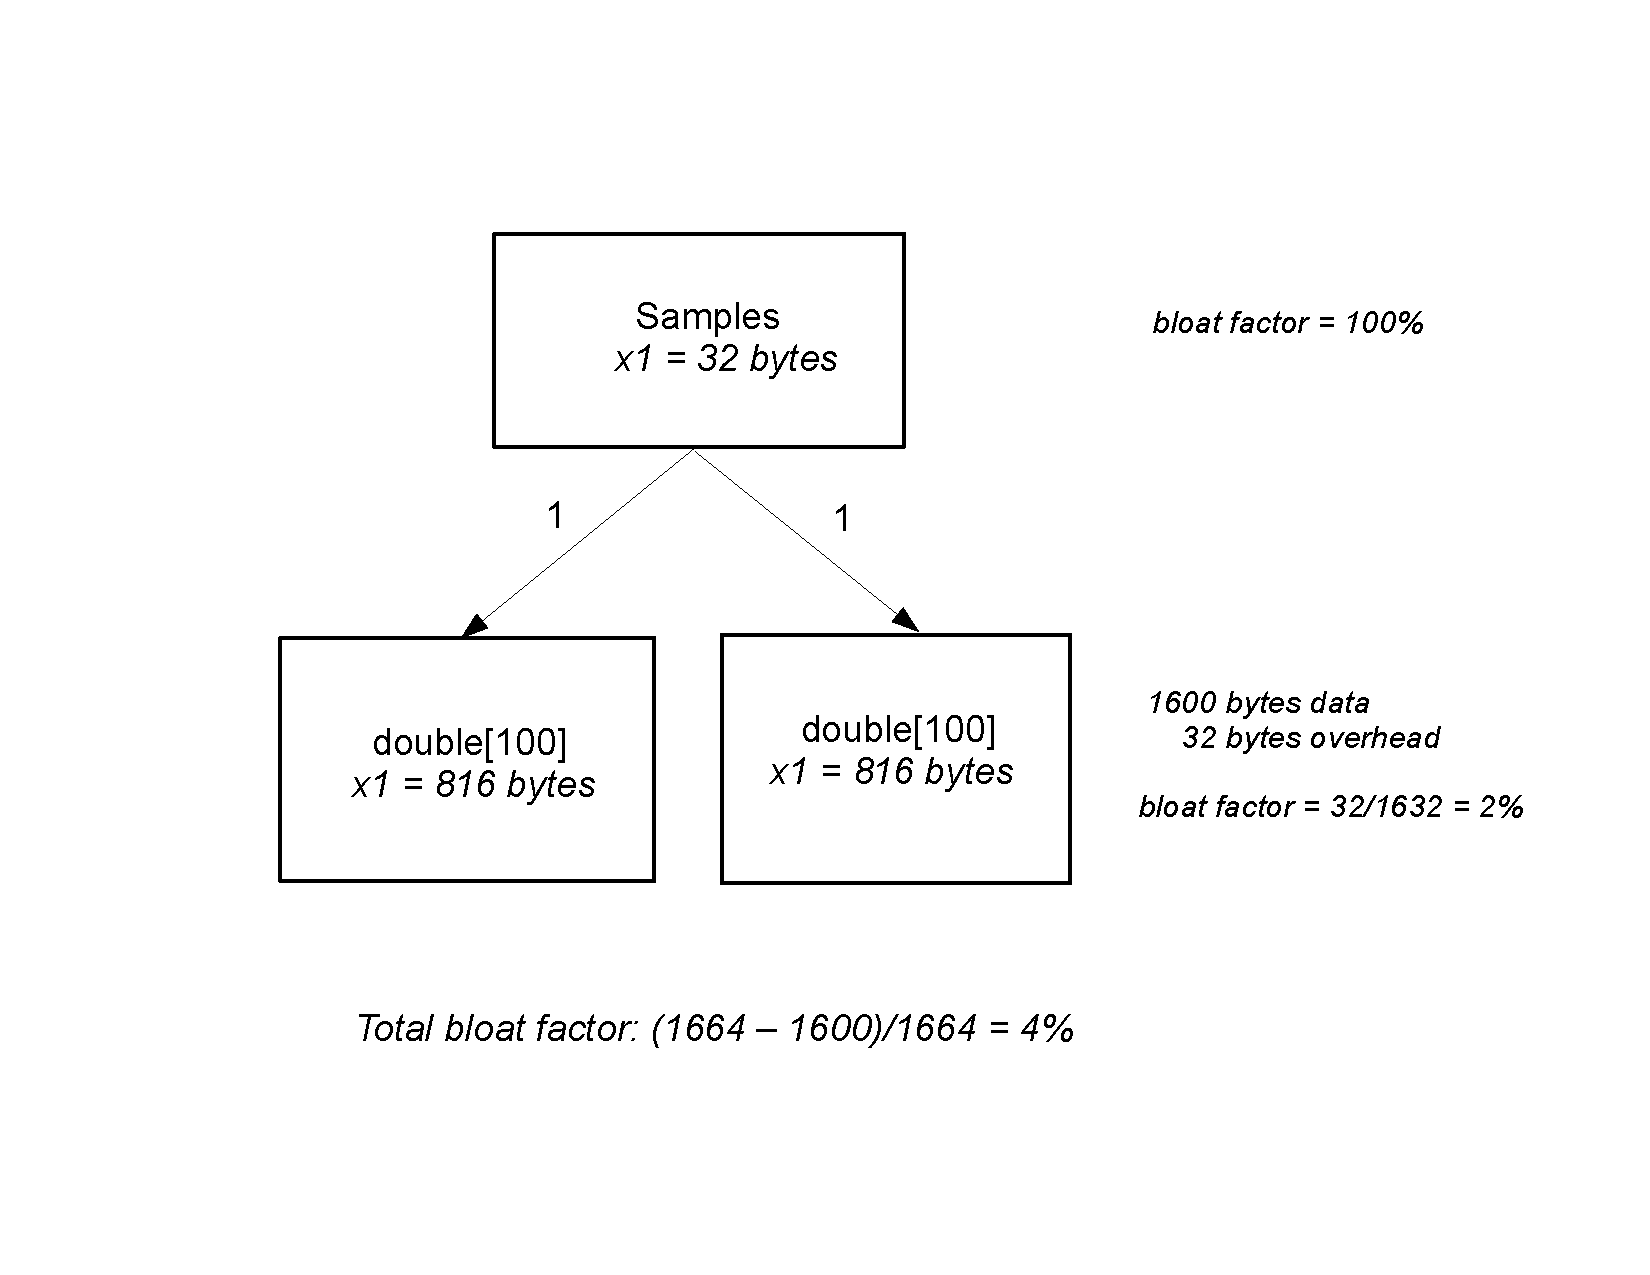
\includegraphics[width=0.7\textwidth]{Figures/chapter3/array-doubles}
  \caption{EC Diagram for 100 samples stored in two parallel arrays}
  \label{fig:content-schematic-arrays-doubles}
\end{figure}

For the three designs presented, there is a tradeoff between ease of programming and memory efficiency. More programming is needed as the design becomes more memory efficient. However, in many cases, memory efficient designs are just as easy to implement as inefficient designs. When there are two distinct execution phases, as in this example, the data structure can be trimmed after the first phase, to eliminate empty space reserved for growth. Another option is to use one data structure in the first phase, and copy it into a second data structure for the second phase. This approach can sometimes be a good compromise between ease-of-programming and memory efficiency.
 
\section{Scalability}
\label{scalability}

The evaluation of the three monitoring system designs was based on only 100 samples. In a real scenario, a monitoring system might have to handle hundreds of thousands, or millions, of samples. Stress testing is usually performed late in a development cycle, when it is very costly to fix a memory footprint problem. Using a memory health approach, it possible to predict how well a data structure design will scale much earlier.
 
\begin{figure}
  \centering
  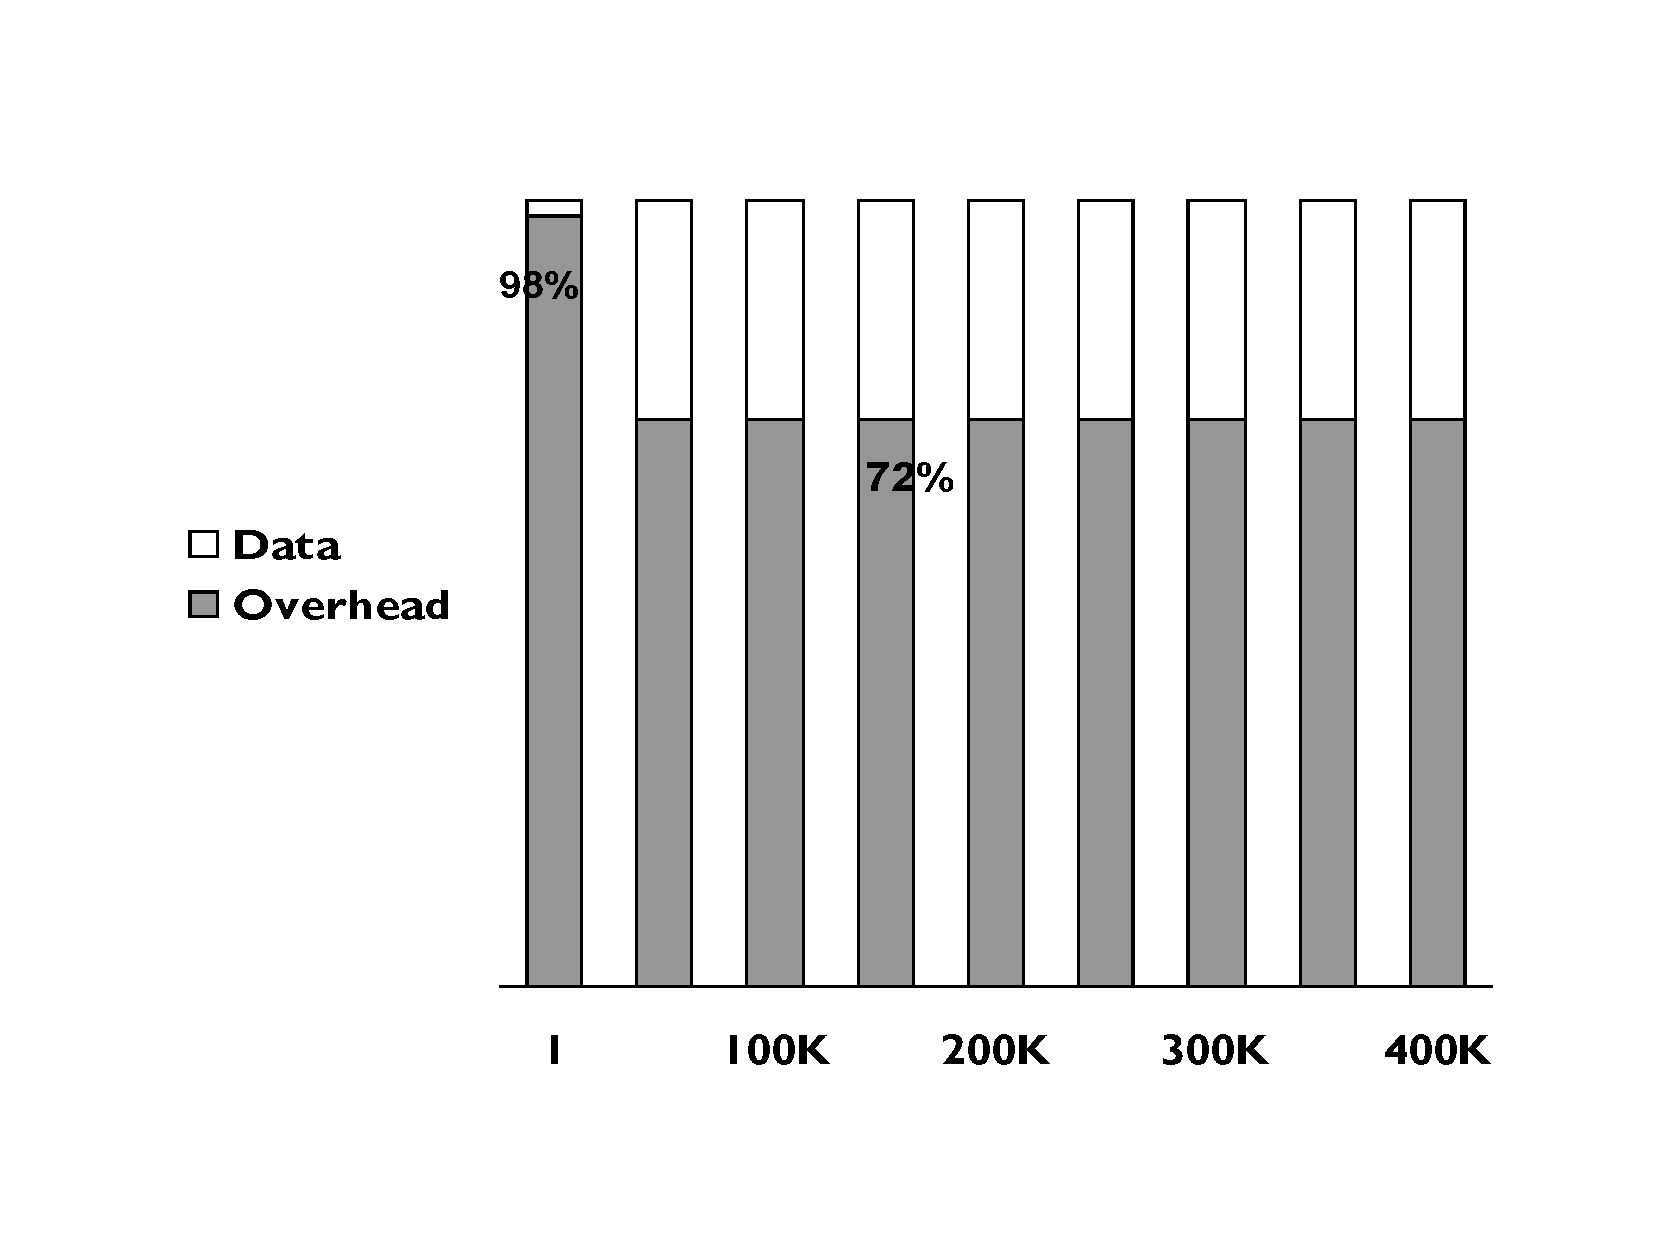
\includegraphics[width=0.7\textwidth]{Figures/chapter3/scalable-health-treemap}
  \caption{Health Measure for the \texttt{TreeMap} Design Shows Poor Scalability}
  \label{fig:scalable-health-treemap}
\end{figure}
The basic question for predicting scalability is what happens to the bloat factor as a data structure grows. The \texttt{TreeMap} design has 74\% overhead with 100 samples. With 100,000 samples, maybe the high overhead will be amortized away, that is, maybe this design will scale well, even if it is inefficient for small data sizes. The bar graph in Figure~\ref{fig:scalable-health-treemap} shows how the \texttt{TreeMap} design scales as the number of samples increase. Each bar is split into two parts: the percentage of overhead and the percentage of data. For a single sample, the overhead is 98\%! As more samples are added, the bloat factor drops to 72\%. Unfortunately, with 200,000 samples, and 300,000 samples, the bloat factor is still 72\%. The \texttt{TreeMap} design is not only bloated, but it also does not scale. It is constantly bloated.

To understand why this happens, recall that the infrastructure of \texttt{TreeMap} is made up of nodes, with two 64-element arrays hanging off of each node. As samples are added, the infrastructure grows, since new nodes and arrays are being created. Also, each additional sample has its own overhead, namely the JVM overhead in each \texttt{Double} object. When the \texttt{TreeMap} becomes large enough, the \textit{per-entry overhead} dominates and hovers around 72\%. The bloat factor is larger when the \texttt{TreeMap} is small. In contrast, for small \texttt{TreeMap}s, the fixed cost of the initial \texttt{TreeMap} infrastructure is relatively big. The \texttt{TreeMap} wrapper object alone is 48 bytes. This initial fixed cost is quickly amortized away as samples are added. 

\callout{callout:fixed-and-per-entry-costs}{Fixed vs Per-Entry Overhead}{
The memory overhead of a collection can be classified as either \textit{fixed} or \textit{per-entry}. Fixed overhead stays the same, no matter how many entries are stored in the collection. Small collections with a large fixed overhead have a high memory bloat factor, but the fixed overhead is amortized away as the collection grows. Per-entry overhead depends on the number of entries stored in the collection. Collections with a large per-entry overhead do not scale well, since per-entry costs cannot be amortized away as the collection grows. 
}

\begin{figure}
  \centering
  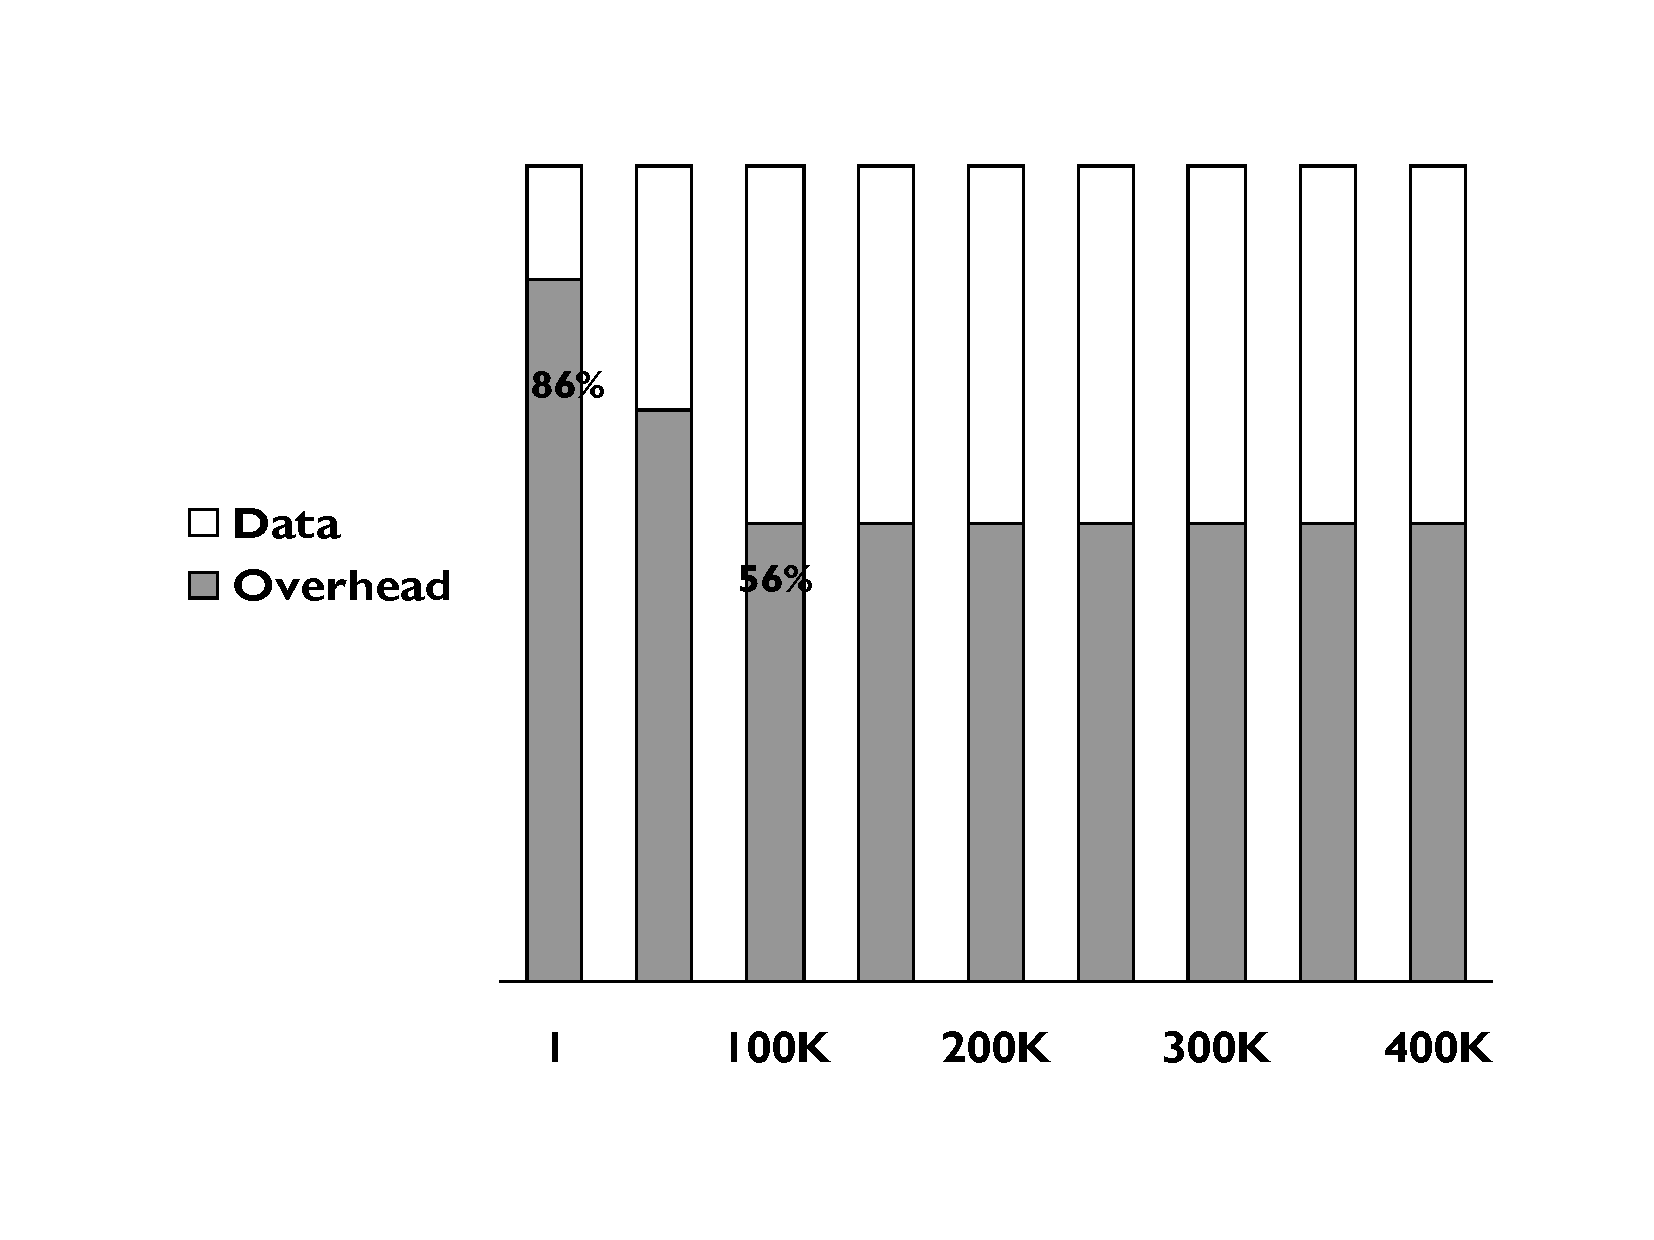
\includegraphics[width=0.7\textwidth]{Figures/chapter3/scalable-health-arraylist}
  \caption{Health Measure for the \texttt{ArrayList} Design }
  \label{fig:scalable-health-arraylist}
\end{figure}

Figure~\ref{fig:scalable-health-arraylist} shows similar data for the \texttt{ArrayList} design. Like the \texttt{TreeMap} design, there is a fixed overhead, which is significant when the \texttt{ArrayList} is small. As the \texttt{ArrayList} grows, the fixed overhead is amortized away, but there is still a per-entry cost of 56\%, that remains constant. 

For the last design that uses arrays, there is only fixed overhead, namely, the \texttt{Samples} object and JVM overhead for the arrays. There is no per-entry overhead at all. Figure~\ref{fig:scalable-health-array} shows the initial 80\% fixed overhead is quickly amortized away. When more samples are added, the bloat factor becomes 0. The samples themselves are pure data.

\begin{figure}
  \centering
  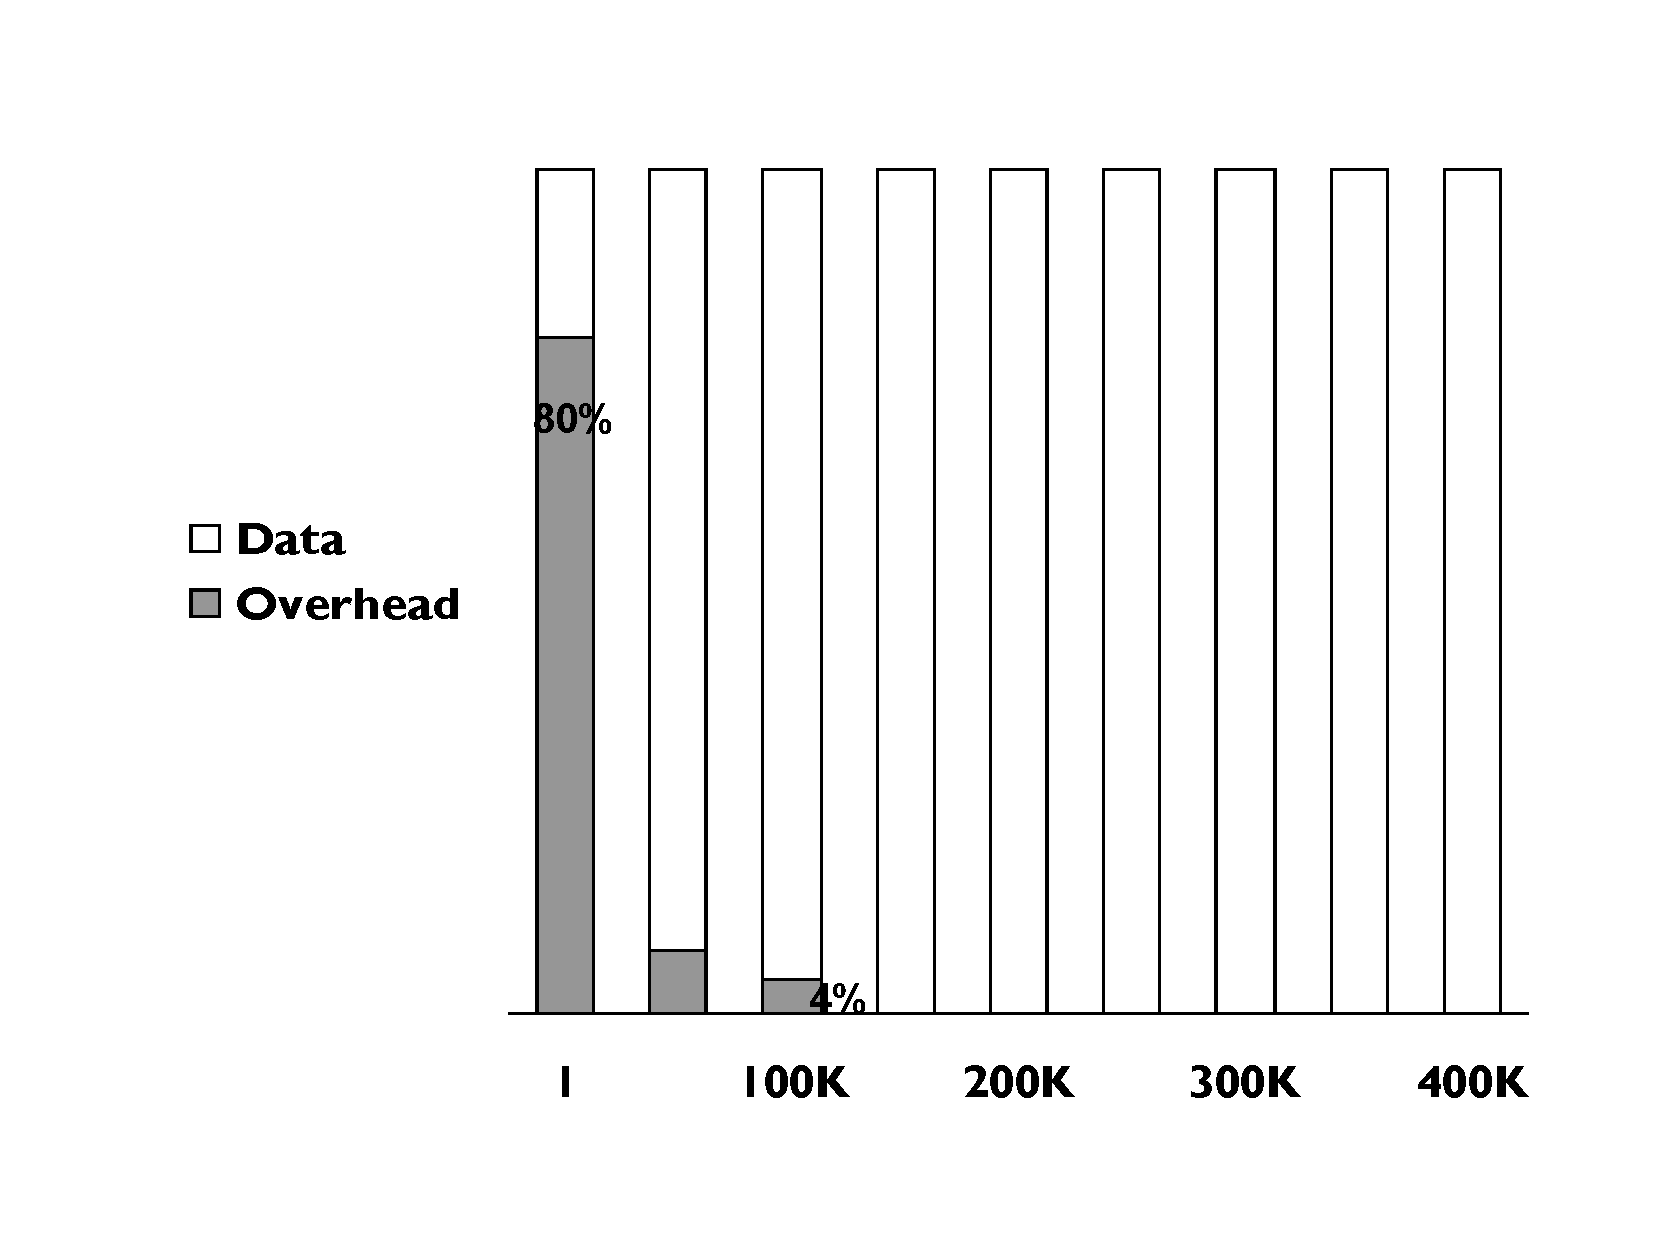
\includegraphics[width=0.7\textwidth]{Figures/chapter3/scalable-health-array}
  \caption{Health Measure for the Array-Based Design Shows Perfect Scalability}
  \label{fig:scalable-health-array}
\end{figure}

This analysis helps predict the memory requirements for large sample sizes. Suppose the monitoring system needs to process 10 million samples. The data alone takes up 160 million bytes (153MB).  The graphs shown in this section can be used to quickly calculate how much memory you will need. For the \texttt{TreeMap} design, the overhead cost is 72\%, so you will need 546MB to store the samples. For the \texttt{ArrayList} design, you will need 347MB. For the \texttt{array} design, you will need only 153MB. As these numbers show, the design choice can make a huge difference.

\section{Summary}

When you are developing a large application, closing your eyes to quantitative considerations and thinking everything is going to be fine is risky. Taking the time to measure the cost and health of your data design can pinpoint problems early on. This chapter described three conceptual tools to help evaluate the memory-efficiency of a design.
\begin{itemize}
\item The \textsl{memory bloat factor} measures how much of your the memory usage of your design is real data, and how much is an artifact of the way you have chosen to represent it. This metric tells you how much room there is for improvement, and if in fact you are paying a reasonable price for what you are getting.
\item Complex data structures are built up from data entities and collections of these entities.  The \textsl{Entity-Collection (EC) Diagram} shows the costs associated with the different parts of a complex data structure. These diagrams help you to compare the memory efficiency of different representation choices.
\item By classifying the overhead of a collection as either \textsl{fixed} or \textsl{per-entry}, you can predict how much memory you will need to store very large collections. Being able to predict scalability is critical to meeting the requirements of larges applications. 
\end{itemize}
These are the basic tools used in the rest of this book. To estimate the cost of an entity, you will need to know how many bytes each primitive type needs, what is the pointer size, and what the JVM overhead is. You will learn how to estimate the cost of entities in Chapter 4. To estimate scalability, you will need to know what the fixed and per-entry costs are for the collection classes you are using. These are given in Chapter 7.

%Nevertheless, you should not throw out all the Java libraries and write everything yourself.  It can also prevent unnecessary optimizations that gain little or nothing. You should perform thought experiments, use limit cases to understand optimal designs, and make back-of-the-envelope calculations.  This requires more work, possibly more prototyping, but the effort will likely pays off. Subsequent chapters discuss more techniques for precise estimation of memory health, and provide the data and overhead costs of common primitives and collections needed to perform estimations. 

\end{document}
